The purpose of this section is to evaluate the empirical
performance and runtime of 2 baseline models
(\textsc{GCN}, \textsc{GCN-SA})
and 2 \textsc{GCN-SA}-based architectures modified
with sparse SA mechanisms 
(\textsc{BigBird}, and \textsc{Exphormer})
to determine whether \textsc{GCN-SA} fitted with sparse SA
mechanisms maintain similar classification performance
whilst reducing runtime.
We present results on $ 8 $ graph datasets of varying
degrees of homophily.
More specifically, we are interested in 2 main quantities:
\begin{enumerate}
  \item Classification accuracy for each model
    evaluated on a $ 60/20/20 $ train/validation/test
    split for each dataset.
  \item Empirical runtime measurements for each model
    and each dataset on 500 epochs.
\end{enumerate}

\subsection{Models and Baselines}
We introduce
\textsc{BigBird} and \textsc{Exphormer} to
\textsc{GCN-SA}'s architecture:

\begin{itemize}
  \item \textsc{GCN-SA+Exphormer}: introduce
  \textsc{Exphormer}'s sparse SA patterns to \textsc{GCN-SA} per subsection 2.4.
  For this experiment we use default hyperparameters:
  $ 5 $-degree expander graphs,
  \texttt{Random-d} expander algorithm,
  and 1 virtual global node.
  \item \textsc{GCN-SA+BigBird}: Employ 
  \textsc{BigBird}'s 
  sparse attention mechanism to \textsc{GCN-SA} per subsection 2.4.
  Again we employ default settings.
\end{itemize}

We compare 2 modified GCN-SA with
sparse SA mechanisms to 2 baselines:
\begin{itemize}
  \item GCN: The graph convolutional nework is the base
  to our modified models. Predictions are made by
  averaging over short-range neighbouring nodes.
  \item GCN-SA: The base model of our sparse SA mechanisms
    as described in subsection 2.3.
\end{itemize}

% The GCN is introduced in
% Subsection 2.2. GCN makes predictions by aggregating local information.
% - GCN
% - GCN-SA
% - GCN-SA + bigbird
% - GCN-SA + exphormer

All parameters and hyperparameters pertaining to \textsc{GCN-SA} 
will be identical across models,
allowing fair testing to clearly 
visualize the discrepancies in results.

% To replace \textsc{GCN-SA}'s
% \textsc{StructureLearning} to 
% \textsc{SparseStructureLearning}:
% $\mathbb{R}^{n \times n} \to
% \mathbb{R}^{n \times d} $,
% we implement Principal Component Analysis (PCA)
% on input features, only retaining required information
% while reducing features size. 

% - Explain really quickly about the datasets we will be using
% - Explain for hyperparameters, we will be using the same as 
%   GCN-SA
% - Random seed is set to 42 for all experiments
% - Number of attention heads is 4


\subsection{Results}
Table 1 illustrates the node classification
accuracy of \textsc{GCN-SA+BigBird} and \textsc{GCN-SA+Exphormer}
against the accuracy of \textsc{GCN} and \textsc{GCN-SA}.
As expected, \textsc{GCN} performs the worst
out of the $ 4 $ models. 
There are no clear implications that sparse SA mechanisms 
reduce the accuracy of \textsc{GCN-SA}.

We expected the models equipped with sparse SA mechanisms
to have reduced epoch runtime. 
However, when comparing with \textsc{GNC-SA}, 
no clear improvements are seen, expecially
some models performed worse on specific datasets like
\textsc{GCN-SA+Exphormer} on citerseer. 

Considering the accuracy of \textsc{GCN-SA}
against \textsc{GCN-SA+BigBird} and \textsc{GCN-SA+Exphormer},
limited differences are seen. On the Cora dataset,
\textsc{GCN-SA} and \textsc{GCN-SA+BigBird} performed exactly 
the same, $(90.6 \pm 0.4)$. Runtime comparisons also dictate
no discrepancies between full SA and sparse SA mechanisms
with \textsc{GCN-SA + BidBird} and \textsc{GCN-SA+Exphormer}
performing practically the same as \textsc{GCN-SA}.

\begin{table}
  \caption{Node classification accuracy}
  \label{tab:sample}
  \setlength\tabcolsep{1.5pt}
  \centering
  \begin{tabular}{l c c c c c c c c c c c }
    \toprule
    \textbf{Method/Dataset} &
    Cora & Cites. & Pubmed & Chame. & 
    Squir. & Corne. & Texas & Wiscon. \\
    \midrule
    \textsc{GCN} &
    87.5$\pm$1.2 & 78.3$\pm$2.1 & 88.2$\pm$0.4 & 60.7$\pm$2.1 &
    42.4$\pm$1.2 & 62.5$\pm$3.6 & 60.9$\pm$5.7 & 60.3$\pm$4.9 \\
    \textsc{GCN-SA} &
    90.6$\pm$0.4 & 79.2$\pm$0.5 & 91.0$\pm$0.6 & 63.8$\pm$2.0  &
    46.8$\pm$1.5 & 91.5$\pm$4.9 & 90.0$\pm$2.4 & 91.0$\pm$2.4 \\
    \textsc{GCN-SA+BBird} &
    90.6$\pm$0.4 & 79.0$\pm$0.6 & 90.8$\pm$0.6 & 64.8$\pm$1.8  &
    46.7$\pm$1.7 & 91.9$\pm$4.2 & 89.4$\pm$2.4 & 91.9$\pm$2.3 \\
    \textsc{GCN-SA+Exph} &
    90.4$\pm$0.4 & 79.0$\pm$0.6 & 91.0$\pm$0.5 & 63.9$\pm$1.9  &
    46.8$\pm$1.7 & 90.1$\pm$4.1 & 90.1$\pm$2.8 & 91.8$\pm$2.3 \\
    \bottomrule
  \end{tabular}
\end{table}

\begin{figure}
  \centering
  % The next line would normally be \includegraphics instead.
  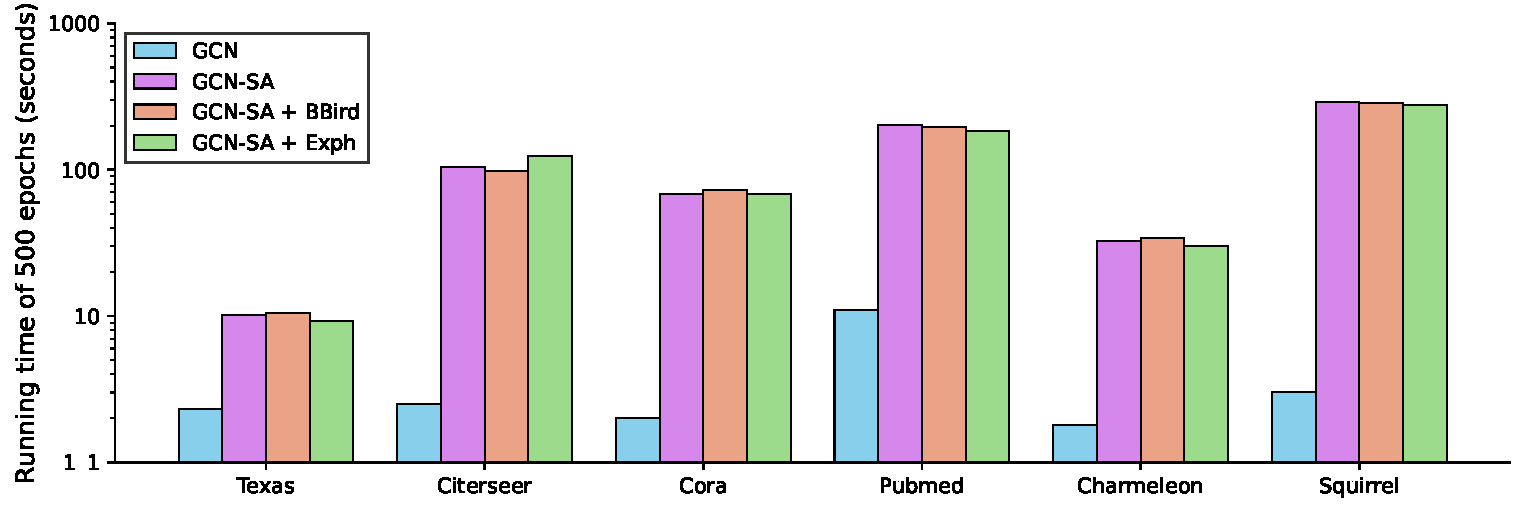
\includegraphics[page=1, width=\linewidth]{src/time_complexity.pdf}
  \caption{Runtime Comparison.}
  \label{fig:sample}
\end{figure}
% \begin{itemize}
%   \item node classification accuracy
%   \item dataset homophily ratios
%   \item model runtime for 500 epochs.
% \end{itemize}

% \begin{itemize}
%   \item Describe each experiment that you did. Say what each experiment is trying to test. 
%   \item Ideally, each experiment should only try to test one thing and you should control for as many other factors as possible. 
%   \item Subsequently, summarize the result of your experiment, in both the text and in a nice visual form such as a figure; in most cases, \textbf{a table with a huge list of numbers is not a nice way to summarize information}.
% \end{itemize}
